\chapter{Equation-to-code map}
\label{app:map}
\begin{figure}[h]
\centering
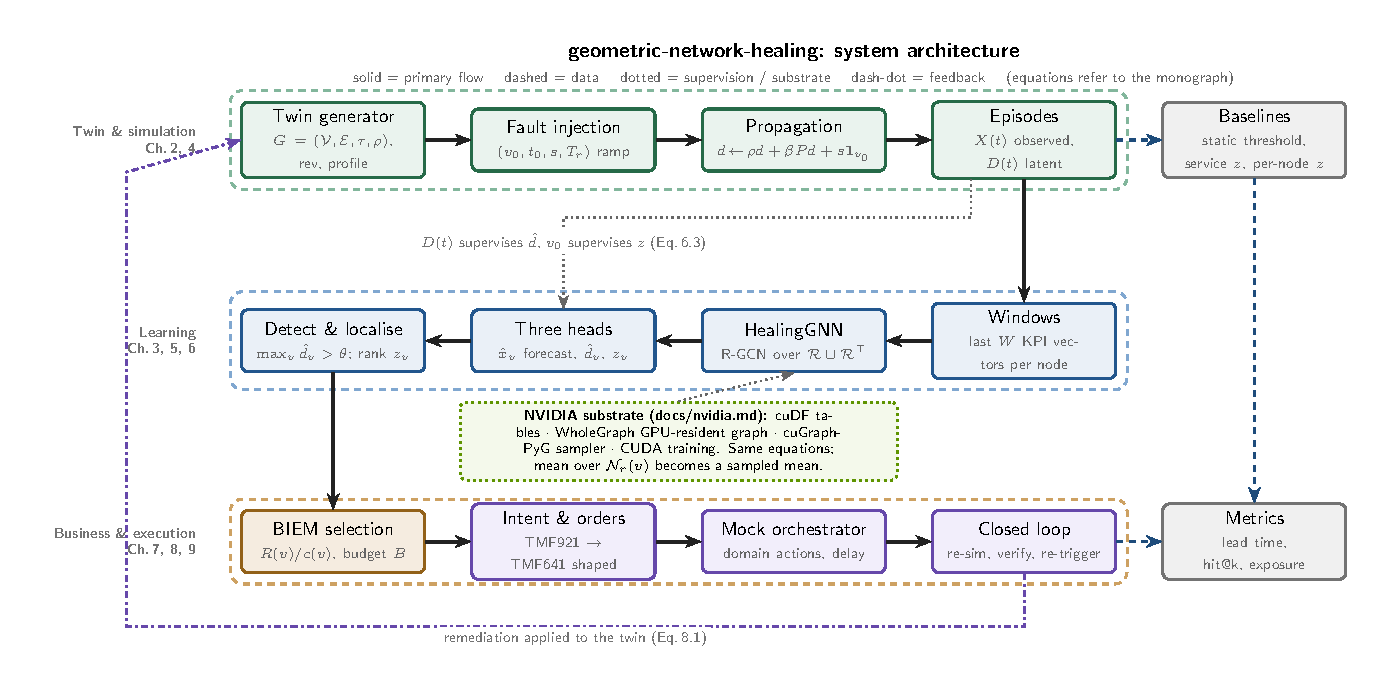
\includegraphics[width=\textwidth]{../design/architecture.pdf}
\caption{System architecture of the repository. Equation numbers refer to this document.}
\end{figure}
\begin{center}
\small
\begin{tabular}{@{}llp{7.2cm}@{}}
\toprule
Equation & Module & Symbol \\
\midrule
\eqref{eq:graph}, \eqref{eq:adjacency}, \eqref{eq:signal} & \code{twin/schema.py}, \code{twin/generator.py} & \code{NodeType}, \code{Relation}, \code{Twin.adjacency()}, \code{Twin.to\_pyg()} \\
\eqref{eq:revenue} & \code{twin/generator.py} & \code{nodes["revenue"]}, \code{Twin.downstream()} \\
\eqref{eq:action}, \eqref{eq:equivariance} & \code{tests/test\_model.py} & numerical equivariance check \\
\eqref{eq:mp}, \eqref{eq:rgcn}, \eqref{eq:input}, \eqref{eq:heads} & \code{gnn/model.py} & \code{HealingGNN} \\
\eqref{eq:injection} & \code{sim/faults.py} & \code{Fault.injection()} \\
\eqref{eq:nominal}, \eqref{eq:observation}, \eqref{eq:propagation} & \code{sim/dynamics.py} & \code{simulate()} \\
\eqref{eq:stability} & \code{tests/test\_twin\_and\_sim.py} & \code{test\_faults\_attenuate\_per\_hop} \\
\eqref{eq:alarm} & \code{baselines/alarms.py} & \code{threshold\_alarm\_detection()}, \code{zscore\_detection()} \\
\eqref{eq:residual}, \eqref{eq:detection} & \code{gnn/detect.py} & \code{calibrate\_threshold()}, \code{detect()} \\
\eqref{eq:forward} & \code{sim/dynamics.py} & implicit in the recursion \\
\eqref{eq:rca} & \code{gnn/detect.py} & \code{rank\_root\_causes()} \\
\eqref{eq:loss} & \code{gnn/train.py} & \code{train()} \\
\eqref{eq:rar}, \eqref{eq:selection} & \code{intent/biem.py} & \code{propose\_branches()}, \code{select\_order()}, \code{to\_tmf921\_intent()} \\
\eqref{eq:exposure} & \code{orchestration/tmf641.py} & \code{closed\_loop()} \\
\eqref{eq:leadtime}--\eqref{eq:triage} & \code{evaluation/metrics.py} & \code{lead\_time()}, \code{hit\_at\_k()}, \code{triage\_reduction()} \\
sampling (Ch.~\ref{ch:nvidia}) & \code{gnn/scale.py} & \code{make\_cugraph\_loader()} \\
\bottomrule
\end{tabular}
\end{center}
